\documentclass[tikz,border=4pt]{standalone}
\usepackage[T1]{fontenc}
\usepackage{lmodern}
\usetikzlibrary{arrows.meta,positioning,fit,backgrounds,calc,shapes.geometric,decorations.pathreplacing}
\begin{document}
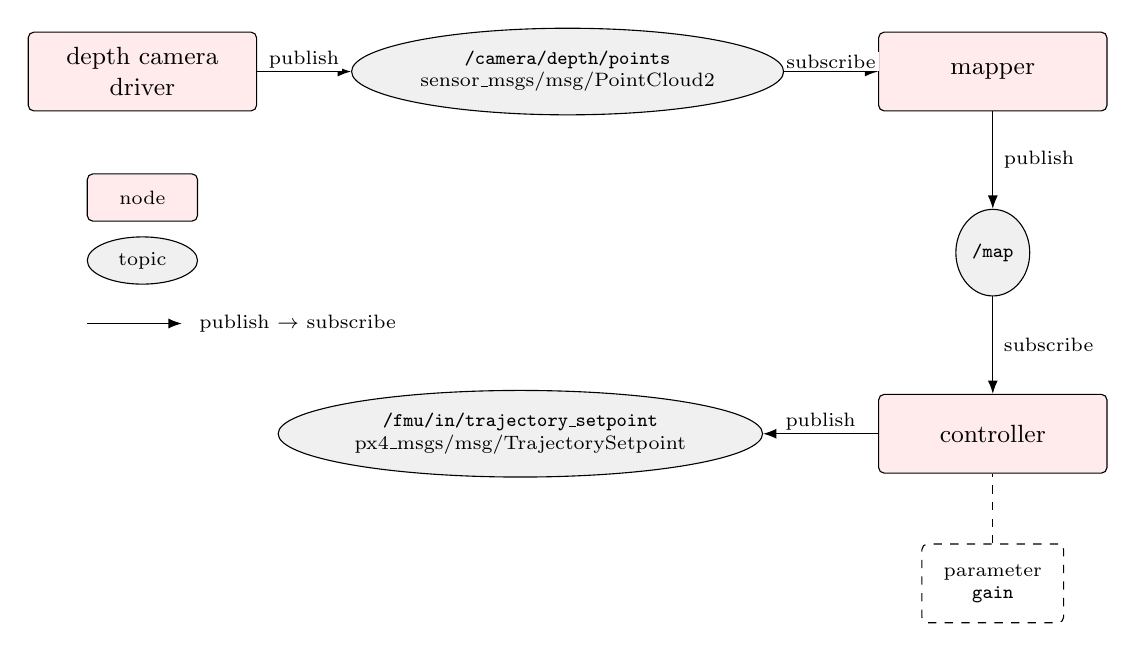
\begin{tikzpicture}[
  blk/.style={draw,rounded corners=2pt,minimum height=10mm,minimum width=29mm,align=center,font=\small,fill=white},
  ros/.style={blk,fill=red!8},
  top/.style={draw,ellipse,minimum height=11mm,align=center,font=\scriptsize,fill=gray!12,inner sep=2pt},
  lab/.style={font=\scriptsize,fill=white,inner sep=1pt,align=center},
  >={Latex}]
\node[ros] (cam) at (0,0) {depth camera\\driver};
\node[top] (t1) at (5.4,0) {\texttt{/camera/depth/points}\\sensor\_msgs/msg/PointCloud2};
\node[ros] (map) at (10.8,0) {mapper};
\node[top] (t2) at (10.8,-2.3) {\texttt{/map}};
\node[ros] (ctl) at (10.8,-4.6) {controller};
\node[top] (t3) at (4.8,-4.6) {\texttt{/fmu/in/trajectory\_setpoint}\\px4\_msgs/msg/TrajectorySetpoint};
\node[blk,dashed,minimum width=18mm,font=\scriptsize] (par) at (10.8,-6.5) {parameter\\\texttt{gain}};
\draw[->] (cam) -- node[lab,above]{publish} (t1);
\draw[->] (t1) -- node[lab,above]{subscribe} (map);
\draw[->] (map) -- node[lab,right,xshift=1mm]{publish} (t2);
\draw[->] (t2) -- node[lab,right,xshift=1mm]{subscribe} (ctl);
\draw[->] (ctl) -- node[lab,above]{publish} (t3);
\draw[dashed] (par) -- (ctl);
\node[ros,minimum height=6mm,minimum width=14mm,font=\scriptsize] at (0,-1.6) {node};
\node[top,minimum height=6mm,minimum width=14mm] at (0,-2.4) {topic};
\draw[->] (-0.7,-3.2) -- (0.5,-3.2);
\node[font=\scriptsize,anchor=west] at (0.6,-3.2) {publish $\rightarrow$ subscribe};
\end{tikzpicture}
\end{document}
